\documentclass{beamer}
\usepackage[spanish]{babel}
\usepackage[utf8]{inputenc}
\usepackage{color}
\usepackage{parskip}
\usepackage{graphicx}
\usepackage{multirow}
\usepackage{listings}
\definecolor{mygreen}{rgb}{0,0.6,0}
\definecolor{lbcolor}{rgb}{0.9,0.9,0.9}


\usetheme{Madrid}

\title{Decorator}

\author{Christofer Fabián Chávez Carazas}

\institute{Universidad Nacional de San Agustín}

\date{\today}

\lstset{
backgroundcolor=\color{lbcolor},
    tabsize=4,    
%   rulecolor=,
    language=[GNU]C++,
        basicstyle=\tiny,
        aboveskip={1.5\baselineskip},
        columns=fixed,
        showstringspaces=false,
        extendedchars=false,
        breaklines=true,
        prebreak = \raisebox{0ex}[0ex][0ex]{\ensuremath{\hookleftarrow}},
        frame=single,
        showtabs=false,
        showspaces=false,
        showstringspaces=false,
        identifierstyle=\ttfamily,
        keywordstyle=\color[rgb]{0,0,1},
        commentstyle=\color[rgb]{0.026,0.112,0.095},
        stringstyle=\color{red},
        numberstyle=\color[rgb]{0.205, 0.142, 0.73},
%        \lstdefinestyle{C++}{language=C++,style=numbers}’.
}

\begin{document}
 
 \begin{frame}
  \titlepage
 \end{frame}

\begin{frame}{Motivación}
  \begin{itemize}
  \item A veces es necesario añadir responsabilidades a objetos individuales, no a una clase entera.
  \item Por ejemplo, cuando un conjunto de herramientas de interfaz gráfica de usuario debe permitir agregar propiedades a cualquier componente.
  \item Una forma de añadir responsabilidades es con la herencia, pero es poco flexible.
  \item La solución está en encapsular dentro de otro objeto, llamado Decorador, las nuevas responsabilidades.
  \end{itemize}
\end{frame}

\begin{frame}{Decorator}
 \begin{itemize}
  \item El decorador redirige las peticiones al componente asociado.
  \item Opcionalmente puede realizar tareas adicionales antes y después de redirigir la petición.
  \item Es transparente para el cliente.
 \end{itemize}
\end{frame}

\begin{frame}{Aplicabilidad}
Este patron se utiliza cuando:
 \begin{itemize}  
    \item se necesita añadir responsabilidades a objetos individuales de forma dinámica y transparente.
    \item se necesita retirar responsabilidades a otros objetos.
    \item la extensión mediante la herencia no es viable.
    \item hay una necesidad de extender la funcionalidad de una clase, pero no hay razones para extenderlo a través de la herencia.
    \item existe la necesidad de extender dinámicamente la funcionalidad de un objeto y quizás quitar la funcionalidad extendida.
 \end{itemize}
\end{frame}

\begin{frame}{Participantes}
  \begin{figure}
   \centering
    
\includegraphics[scale=0.4]{1.jpg}
  \end{figure}
\end{frame}

\begin{frame}{Ventajas}
\begin{itemize}
 \item Mayor flexibilidad que la herencia estática.
 \item Evita las clases cargadas de características, ya que permite la adición de responsabilidades.
 \item Son fáciles de personalizar por aquellos que entienden su estructura. 
\end{itemize}
\end{frame}

\begin{frame}{Desventajas}
\begin{itemize}
 \item Un decorador y su componente no son idénticos. Un decorador actúa como una caja transparente, pero desde el punto de vista de la identidad del objeto un componente decorado no es idéntico a la del propio componente.
 \item Un diseño que utiliza Decorator a menudo resulta en sistemas compuestos por gran cantidad de pequeños objetos parecidos. Los objetos sólo se diferencian en la manera en que están interconectados. Esto puede resultar difícil de aprender y depurar.
 \end{itemize}	
\end{frame}

\begin{frame}{Implementación}
 \begin{itemize}
  \item La interfaz de un objeto decorador debe ajustarse a la interfaz del componente que decora (por herencia).
  \item Omitiendo la clase Decorador abstracta. No hay necesidad de definir una clase Decorador abstracta cuando sólo tiene que añadir una responsabilidad.
 \end{itemize}
\end{frame}

\begin{frame}{Implementación}
 \begin{itemize}
  \item Componentes livianos. Es importante mantener la clase Component liviana para evitar que los decoradores resulten demasiado cargados, es decir, debe centrarse en la definición de una interfaz, no en el almacenamiento de datos (quienes deberían ser tratados en subclases).
  \item Decoratos vs Strategy: son dos formas alternativas de cambiar un objeto. El patrón Decorador sólo cambia un componente desde el exterior, de modo que los decoradores son transparentes para el componente. Con Strategy, el componente conoce las posibles extensiones, teniendo que hacer referencia y mantener las correspondientes estrategias.
 \end{itemize}
\end{frame}

\defverbatim[colored]\lstVC{
\begin{lstlisting}
  class VisualComponent{
  public:
    VisualComponent();
    virtual void Draw();
    virtual void Resize();
   //...
  };
\end{lstlisting}
}

\defverbatim[colored]\lstD{
\begin{lstlisting}
 class Decorator:public VisualComponent{
 public:
    Decorator(VisualComponent*);
    virtual void Draw();
    virtual void Resize();
    //...
 private:
    VisualComponent* component;
 };
\end{lstlisting}

}


\begin{frame}{Código}
\textbf{Visual Component:}
 \lstVC
\textbf{Decorator:}
 \lstD
\end{frame}

\defverbatim[colored]\lstDD{
\begin{lstlisting}
 void Decorator::Draw(){
  component->Draw();
 }
 
 void Decorator::Rezise(){
  component->Rezise();
 }
\end{lstlisting}

}

\defverbatim[colored]\lstBD{
\begin{lstlisting}
 class BorderDecorator:public Decorator{
 public:
  BorderDecorator(VisualComponent*, int borderWidth);
  virtual void Draw();
 private:
  int _width;
  void DrawBorder(int);
 };
 
 void BorderDecorator::Draw(){
  Decorator::Draw();
  DrawBorder(_width);
 }
\end{lstlisting}

}


\begin{frame}{Código}	
 \lstDD
 \textbf{Border Decorator}
 \lstBD
\end{frame}

\begin{frame}
 \begin{figure}
  \centering
  
\includegraphics[scale=0.35]{2.jpg}
 \end{figure}

\end{frame}

\begin{frame}
 \begin{figure}
  \centering
  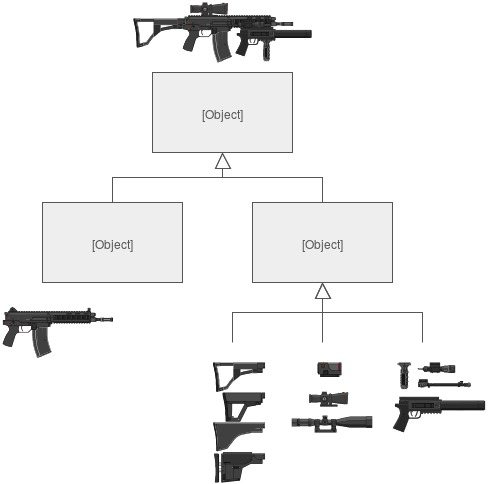
\includegraphics[scale=0.5]{3.jpg}
 \end{figure}
\end{frame}


\begin{frame}{Patrones Relacionados}
 \begin{itemize}
  \item \textbf{Adapter:} un Decorator sólo cambia las responsabilidades de un objeto, mientras que un adaptador dará a un objeto una interfaz nueva.
  \item \textbf{Composite:} un Decorator puede ser visto como un composite de un solo componente. Sin embargo, un decorador añade responsabilidades adicionales.
  \item \textbf{Strategy:} un Decorator permite cambiar la "piel" de un objeto, mientras que un Strategy le permite cambiar las "tripas" (por dentro).
 \end{itemize}
\end{frame}

\begin{frame}{Conclusiones}
 \begin{itemize}
  \item El Decorator es un patron de diseño fácil de aprender.
  \item Ayuda mucho en crear dinamismo.
  \item Puede hasta llegar a eliminar la herencia multiple.
 \end{itemize}
\end{frame}


\begin{frame}{Bibliografía}
  \begin{thebibliography}{10}
  \beamertemplatebookbibitems
    \bibitem{Libro}
    Ralph Johnson, Erich Gamma, John Vlissides, Richard Helm
    \newblock Design Patterns: Elements of Reusable Object-Oriented Software
    \newblock Addison-Wesley, 1995
   \end{thebibliography}
\end{frame}
 
\end{document}
